\section{General comments}

\subsection*{Reviewer comment 1}

As noted in Section 4.2.4, the a priori assumptions do not describe reality very
well. In particular, I suspect that the information content of Dm and N0* is
highly dependent on the a priori assumptions of these two variables in the
retrieval framework. Especially with a radar measurement, since Z is sensitive
to both parameters over a wide range of the parameter space, the relative
sensitivity and therefore information content will almost entirely depend on the
relative constraints on these parameters imposed by Xa and Sa. As such it is
imperative to accurately characterize these. I understand the choice to use the
DARDAR constraints, but it’s clear from the cross-section plots that the model
ice particle concentrations vary over a much wider range than the roughly 2
orders of magnitude that Eq. 4 provides over a 220-272 K temperature range. So,
when the retrieval results are compared to model “reality”, it seems that a lot
of N0* variability is folded into Dm and this is especially evident in Figures
13 and 14. My overall concern is that it is difficult to interpret some of the
results when the model fields and the a priori assumptions differ so strongly.

\subsubsection*{Author response}

To avoid potential misunderstanding we would like to point out that the
variation of the a priori mean with temperature, which is given by Eq. 4, does
not limit the retrieved values of $N_0^*$ to this range. How much $N_0^*$ is
allowed to vary around the a priori mean is determined by the covariance matrix.
Since the standard deviation for $\text{log}_{10}(N_0^*)$ at each grid point was
set to $2$ (c.f. Tab.~3), $N_0^*$ is free to vary over several orders of
magnitude in addition to the variation of the a priori profile.

Furthermore, the sentence in Section~4.2.4 was badly formulated and did not
really express what we wanted to say there. The a priori assumptions are not
generally bad for the model (after all the averaged results for the first scene
are good). Rather, they are insufficient to accurately describe the
(co-)variability of $D_m$ and $N_0^*$.

Nonetheless, the point raised by the reviewer certainly remains valid: In
absolute terms, the interpretation of the retrieval results is dependent on the
a priori assumptions. We argue here, however, that by applying equivalent a
priori assumptions in all retrievals, we can still derive conclusions on the
benefits of the combined retrieval approach based on a relative interpretation
of the retrieval results. Our results indicate that the combined retrieval has
to rely less on a priori assumptions than the radar-only retrieval. This is
an important advantage of the combined retrieval since if $D_m$ and $N_0^*$
could be constrained reliably a priori we would not have the uncertainties in
the observational record of ice hydrometeors that we see today.

\subsubsection*{Changes in manuscript}

\begin{itemize}
\item The discussion of the role of the a priori and its impact on results has
  been extended by adding the following paragraph to the manuscript:

  \begin{change}[491]
\DIFadd{The a priori assumptions used in this study were chosen similar to those of the
DARDAR-CLOUD product, since they represent well established and validated
assumptions for ice cloud retrievals. The role of the a priori is to complement
the observations with additional information required to make the retrieval
problem tractable. For the hydrometeor retrieval this means that the a priori
determines how information from the observations, which alone is insufficient to
determine both degrees of freedom of the PSD, is distributed between its $D_m$
and $N_0^*$ parameters. For the radar-only retrieval, this works well for cloud
systems containing both ice and snow but leads to biased retrievals of both IWC
and IWP when this is not the case (}\DIFaddend Fig.~\ref{fig:boxes}\DIFdelbegin \DIFdel{. In general, the passive-only and the combined retrievals display }\DIFdelend \DIFaddbegin \DIFadd{). The DARDAR product
uses co-located lidar observations to resolve the ambiguity where observations
from both sensors are available. As our results show, this can be achieved also
by combining a radar with passive microwave radiometers. However, while the
overlap between lidar and radar is restricted to relatively thin clouds,
microwave radiometers can provide sensitivity even deeper inside clouds.
}
  \end{change}

\item The following paragraph has been added to the discussion of the limitations of
  the study which clearly states that the retrieval results should not be
  interpreted in absolute terms:

  \begin{change}[549]
  \DIFadd{An important limitation of this study is its scope: The aim here was not to
  develop a production-ready combined retrieval product but rather a
  proof-of-concept to explore this observational approach. The retrieval results
  presented here should therefore not be interpreted in absolute terms. The
  primary results are based on the relative performances of the three retrieval
  methods: Given equivalent }\DIFaddend a priori assumptions\DIFdelbegin \DIFdel{do
  not describe reality very well. In addition to that, the current implementation
  of the retrieval is computationally very expensive. For further development of
  the combined retrieval
  concept it may therefore be advisable to revisit the applied retrieval method in search for a potentially more suitable alternative}\DIFdelend \DIFaddbegin \DIFadd{, the combined retrieval
  demonstrates higher sensitivity to the microphysical properties than the
  radar-only retrieval and lower errors in terms of IWC than the passive-only
  retrieval}\DIFaddend .
  \end{change}

\item The paragraph starting on line 524 on the limitations of the OEM as
  retrieval method has been removed since its interpretation caused confusion
  and it was deemed to be of minor importance for the overall results of the study.
  \end{itemize}

\subsection*{Reviewer comment 2}

Forward model error is introduced when the different species present in the
model microphysics are combined into one species and when different scattering
models are used to represent the ice particles. That this is not represented in
Se could lead to over-fitting and poor convergence (I suspect this is part of
the reason why the normalized cost is much higher for the radiometer-including
retrievals). It should be relatively easy to quantify this error by re-running
the simulations with the retrieval assumptions(combining ice species, different
scattering models), and I suspect that this error term would dominate the
instrument noise term for many channels.

\subsubsection*{Author response}

It is certainly true that the simplified forward model used in the retrieval
introduces a forward modeling error and that it will likely dominate the sensor
noise. However, we do not agree with the reviewer that this error is easy to
quantify. First of all, the error will not be Gaussian and will depend on the
cloud composition and the assumed particle shape, so that a more sophisticated
error model would be required to describe the error accurately. Fitting such a
model to the test scenes would likely yield overly optimistic results as this
would mean making use of information which would not be available
for a real retrieval scenario.

Because of these difficulties, we decided to not pursue this approach in the
study. However, since this is an important point to mention, we will add a
paragraph on this issue in the discussion.

\subsubsection*{Changes in manuscript}

\begin{change}[513]
\DIFaddbegin \DIFadd{It should be noted, that none of the presented
  retrievals accounts for the error caused by the simplified forward model and
  the choice of the particle model. This has not been pursued here because of
  the difficulty of fitting a suitable model to the forward model errors which
  are likely non-Gaussian and scene-dependent. However, it is likely that
  accounting for these errors can improve retrieval performance and weaken the
  impact of the particle choice on the retrieval results}\DIFaddend .
\end{change}

\section{Specific comments}

\subsection*{Reviewer comment 1}
Lines 85-88: I recommend the use of geographical spatial references
(i.e.,north/south rather than left/right)

\subsubsection*{Author response}

The proposed change has been adopted in the revised version of the manuscript.

\subsubsection*{Changes in manuscript}

\begin{change}[85]
The first test scene, shown in panel (a), is located in the tropical
Pacific and contains a \DIFdelbegin \DIFdel{convective storm }\DIFdelend \DIFaddbegin \DIFadd{mesoscale convective }\DIFaddend system in the \DIFdelbegin \DIFdel{right }\DIFdelend \DIFaddbegin \DIFadd{northern }\DIFaddend half of the scene
and its anvil which extends into the \DIFdelbegin \DIFdel{left halfof the scene}\DIFdelend \DIFaddbegin \DIFadd{southern half}\DIFaddend . The second scene, shown in
panel (b), is located in the North Atlantic and contains an ice cloud in the
\DIFdelbegin \DIFdel{first quarter }\DIFdelend \DIFaddbegin \DIFadd{southern part }\DIFaddend and a low-level, mixed-phase cloud in the \DIFdelbegin \DIFdel{remainder of the
scene}\DIFdelend \DIFaddbegin \DIFadd{northern part}\DIFaddend .
\end{change}

\subsection*{Reviewer comment 2}

Line 98 (also 176,252,449): Instead of vertical/horizontal (which are
dependent on the convention used for plotting), I recommend the use of
concentration/size tocharacterize the dimensions of the particle size
distribution.

\subsubsection*{Author response}

The proposed change has been adopted in the revised version of the manuscript.

\subsubsection*{Changes in manuscript}

\begin{change}[95]
The \DIFdelbegin \DIFdel{four panels display the prognosed particle size
distributions for the four frozen hydrometeor types together with renderings of
the particle shapes used in the forward simulations. As these plots show, the
}\DIFdelend assumed particle size distributions across
different ice species vary mostly in their \DIFdelbegin \DIFdel{horizontal and vertical scaling }\DIFdelend \DIFaddbegin \DIFadd{scaling with respect to size and
  concentration}\DIFaddend , whereas the \DIFdelbegin \DIFdel{function }\DIFdelend \DIFaddbegin \DIFadd{normalized }\DIFaddend shape shows less variability.
\end{change}

\begin{change}[175]

\DIFadd{The PSDs of frozen hydrometeors and rain }\DIFaddend are represented
using the normalized particle size distribution formalism proposed by
\cite{delanoe05}. The PSD of a hydrometeor species at a given \DIFdelbegin
\DIFdel{height level is represented by a vertical and a horizontal scaling
  parameter, the }\DIFdelend \DIFaddbegin \DIFadd{altitude is modeled using a
  generalized gamma distribution function with four parameters. The }\DIFaddend
mass-weighted mean diameter $D_m$\DIFaddbegin \DIFadd{, which scales the PSD
  along the size dimension, }\DIFaddend and the normalized number density
$N_0^*$\DIFdelbegin \DIFdel{. Alternative parametrizations using mass density
  and $D_m$ or the mass density and $N_0^*$ have been tested but no considerable
  effect on retrieval performance has been observed. }%DIFDELCMD <

%DIFDELCMD < %%%
\DIFdel{The retrieval computes vertical profiles of the two scaling parameters
  $D_m$ and $N_0^*$ for each of the two hydrometeor species. The remaining shape
  of each PSD is described by the shape parameters $\alpha$ and $\beta$, not to
  be confused with the parameters of the mass-size relationship shown in
  Tab.~1. The shape parameters are set to fixed,
  species-specific values. This principle is illustrated in
  Fig.~3. The plot displays the a-priori-assumed shapes
  of the particle size distribution of frozen and liquid hydrometeors. The
  retrieved horizontal and vertical scaling parameters }\DIFdelend ,
\DIFdelbegin \DIFdel{$D_m$ and $N_0^*$, are used as units for the axes of the
  plot so that }\DIFdelend \DIFaddbegin \DIFadd{which scales the particle
  concentration, are the two retrieved degrees of freedom of the PSD. The other
  two parameters describe }\DIFaddend 

\end{change}


\begin{change}[252]
\DIFdel{In the figure, the cloud signal is displayed in $D_m$-mass density space and
thus shows how the measured passive cloud signal varies with the horizontal and
vertical scaling parameters of
the PSD.
Overlaid onto }\DIFdelend \DIFaddbegin \DIFadd{The cloud signal in the radiometer observations is the
difference between the cloudy- and clear-sky brightness temperatures ($\Delta
T_B$). The signal in the active observations is here defined as the maximum of
the measured profile of radar reflectivity $\text{dBZ}_\text{max}$.
Figure~9 displays }\DIFaddend the contours of \DIFdelbegin \DIFdel{the
passive cloudsignal are the isolines of the maximum radar reflectivity returned
from the cloud ...}\DIFdelend

\end{change}

\begin{change}[449]
The results \DIFdelbegin \DIFdel{show }\DIFdelend \DIFaddbegin \DIFadd{indicate }\DIFaddend that the combined
observations can \DIFdelbegin \DIFdel{simultaneously constrain the horizontal and vertical scaling of }\DIFdelend \DIFaddbegin \DIFadd{constrain }\DIFaddend the \DIFdelbegin \DIFdel{particle size distribution}\DIFdelend \DIFaddbegin \DIFadd{size and concentration of particles in the cloud}\DIFaddend .
\end{change}



%The proposed changes will be adopted in the revised version of the manuscript
%by introducing the following changes:
%
%\begin{change}[97]
%\ldots simulations. As these plots show, the
%assumed particle size distributions across different ice species vary mostly in
%their \DIFdelbegin \DIFdel{horizontal and vertical scaling }\DIFdelend \DIFaddbegin \DIFadd{scaling with respect to size and concentration}\DIFaddend , whereas the function \ldots
%\end{change}
%
%\begin{change}[176]
%The PSD of a hydrometeor species at a \DIFdelbegin \DIFdel{given }\DIFdelend \DIFaddbegin \DIFadd{certain }\DIFaddend height level is
%\DIFdelbegin \DIFdel{represented by a vertical and a horizontal scaling parameter}\DIFdelend \DIFaddbegin \DIFadd{given by a generalized gamma distribution function with four parameters. Two of
%them}\DIFaddend , the mass-weighted mean diameter $D_m$\DIFaddbegin \DIFadd{, which scales the PSD along the size
%dimension, }\DIFaddend and the normalized number density $N_0^*$\DIFdelbegin \DIFdel{. Alternative 
%parametrizations using mass density and $D_m$ or the mass density and $N_0^*$
%have been tested but no considerable effect on retrieval performance has been
%observed.
%}%DIFDELCMD < 
%
%%DIFDELCMD < %%%
%\DIFdel{The retrieval computes vertical profiles of the two scaling parameters $D_m$ and
%$N_0^*$ for each of the two hydrometeor species. The remaining shape of each }\DIFdelend \DIFaddbegin \DIFadd{, which scales the particle
%  concentration, are retrieved. The \ldots}\DIFaddend
%\end{change}
%
%\begin{change}[252]
%The question that is addressed here is whether the combination of active and
%passive observations is able to constrain both the \DIFdelbegin \DIFdel{horizontal and the
%vertical scaling factors of the PSD }\DIFdelend \DIFaddbegin \DIFadd{size and concentration }\DIFaddend of the
%ice particles in the cloud. 
%\end{change}
%
%\begin{change}[449]
%The results show that the combined
%observations can simultaneously constrain the \DIFdelbegin \DIFdel{horizontal and vertical scaling of
%the particle size distribution}\DIFdelend \DIFaddbegin \DIFadd{size and concentration of
%particles in the cloud}\DIFaddend .
%\end{change}


\subsection*{Reviewer comment 3}

Line 100: A few more details on the Milbrant and Yau microphysics sheme that are
relevant to this study would be helpful here. For example: What is the assumed
shape(functional form) of the particle size distribution, and what are the
prognostic variables(e.g., number concentration, mixing ratio)?

\subsubsection*{Author response}

We followed the reviewers comment and added the requested information
to the manuscript.

\subsubsection*{Changes in manuscript}

\begin{change}[89]
The GEM model uses \DIFaddbegin \DIFadd{a two-moment scheme with }\DIFaddend six
types of hydrometeors to represent clouds and precipitation
\citep{milbrandtyau05}: Two classes of liquid hydrometeors (rain and liquid
cloud) and four of frozen hydrometeors (cloud ice, snow, hail and graupel). The
particle size distribution (PSD) of each hydrometeor \DIFdelbegin \DIFdel{type
  is parametrized by its particle number concentration and mass density. The
  full particle size distribution can be prognosed from the two moments using a
  species-dependent parametrization and mass-size relationship. The }\DIFdelend
\DIFaddbegin \DIFadd{class is described by a three-parameter gamma distribution.
  The prognostic parameters of the model are the slope and intercept }\DIFaddend
parameters of the \DIFdelbegin \DIFdel{mass-size relationship are given in
  Tab.~1. As shown in the table, }\DIFdelend
\DIFaddbegin \DIFadd{PSD, which are derived from the predicted mixing ratios and
  number concentrations. The third parameter, which defines the shape of
}\DIFaddend the \DIFdelbegin \DIFdel{masses of all ice particles in the model
  are assumed to scale with a power of three, which leads to high densities for
  large particles. }\DIFdelend \DIFaddbegin \DIFadd{PSD, is set to a fixed,
  species-specific value. For each hydrometeor species a specific mass-size
  relationship is assumed. }\DIFaddend
\end{change}

%To address the reviewers comment, the paragraph describing the Milbrandt-Yau microphysics scheme
%has been extended to provided the information demanded by the reviewer:
%
%\begin{change}[91]
%The GEM model uses \DIFaddbegin \DIFadd{a two-moment scheme with }\DIFaddend six types of hydrometeors to
%represent clouds and precipitation \citep{milbrandtyau05}: Two classes of liquid
%hydrometeors (rain and liquid cloud) and four of frozen hydrometeors (cloud ice,
%snow, hail and graupel). The particle size distribution (PSD) of each
%hydrometeor \DIFdelbegin \DIFdel{type is parametrized by its particle number concentration and mass density. The
%full
%particle size distributioncan be prognosed from the two moments using a
%species-dependent parametrization and
%}\DIFdelend \DIFaddbegin \DIFadd{class is described by a three-parameter gamma distribution. The
%prognostic parameters of the two-moment scheme are the slope and intercept
%parameters of the distribution, which are derived from the mixing ratios and
%number densities predicted by the GEM model. The third parameter of the PSD and
%the }\DIFaddend mass-size relationship \DIFaddbegin \DIFadd{of each hydrometeor class are set to fixed,
%class-specific values}\DIFaddend . The parameters of the mass-size \DIFdelbegin \DIFdel{relationship }\DIFdelend \DIFaddbegin \DIFadd{relationships }\DIFaddend are given
%in Tab.~\DIFdelbegin \DIFdel{\ref{tab:species_parameters}. As
%shown in the table, the }\DIFdelend \DIFaddbegin \DIFadd{\ref{tab:partice_properties}. The }\DIFaddend masses of all ice particles in the
%model are assumed to scale with a power of three, which leads to high densities
%for large particles.
%\end{change}

\subsection*{Reviewer comment 4}
Line 135: Does the ARTS radar solver also provide analytic Jacobians?

\subsubsection*{Author response}

Yes, it does. A sentence will be added to the description of the forward model
to clarify this.

\subsubsection*{Changes in manuscript}
\begin{change}[135]
Radar reflectivities are computed using ARTS' built-in single-scattering radar
solver\DIFaddbegin \DIFadd{, which provides analytic Jacobians}\DIFaddend .
\end{change}
%This is now also mentioned in the description of the retrieval forward model:

%\begin{change}[135]
%All simulations presented in this study were performed using Version 2.3.1245 of
%the Atmospheric Radiative Transfer Simulator (ARTS, \cite{arts18}). Radar
%reflectivities are computed using ARTS' built-in single-scattering radar solver\DIFaddbegin \DIFadd{,
%which provides analytic Jacobians}\DIFaddend . For \ldots
%\end{change}

\subsection*{Reviewer comment 5}
Line 187: “particles” should be “particle”

\subsubsection*{Author response}

The sentence has been removed in the revised version of the manuscript since
the information it conveyed was deemed irrelevant.

%\begin{change}[187]
%  \ldots rain drops. \DIFdelbegin \DIFdel{All calculations involving particles
%    size distributions use the volume-equivalent diameter $D_\text{eq}$ as size
%    variable.
%}%DIFDELCMD < 
%\end{change}


\subsection*{Reviewer comment 6}
Line 198: Is Dm also only retrieved at these 10 points, or just N0* (and Dm retrieved in each radar range gate as in Grecu et al. 2016)?

\subsubsection*{Author response}

$D_m$ is actually retrieved at the resolution of the GEM model scenes. Since
questions about the retrieval grids were raised also by the other reviewers, we
will add an illustration of the grids applied in the different retrieval
configurations to the manuscript.

\subsubsection*{Changes in manuscript}
The figure shown in Fig.~\ref{fig:retrieval_sketch} has been added to the
manuscript to clarify which variables are retrieved at which resolutions.

\begin{figure}
\centering 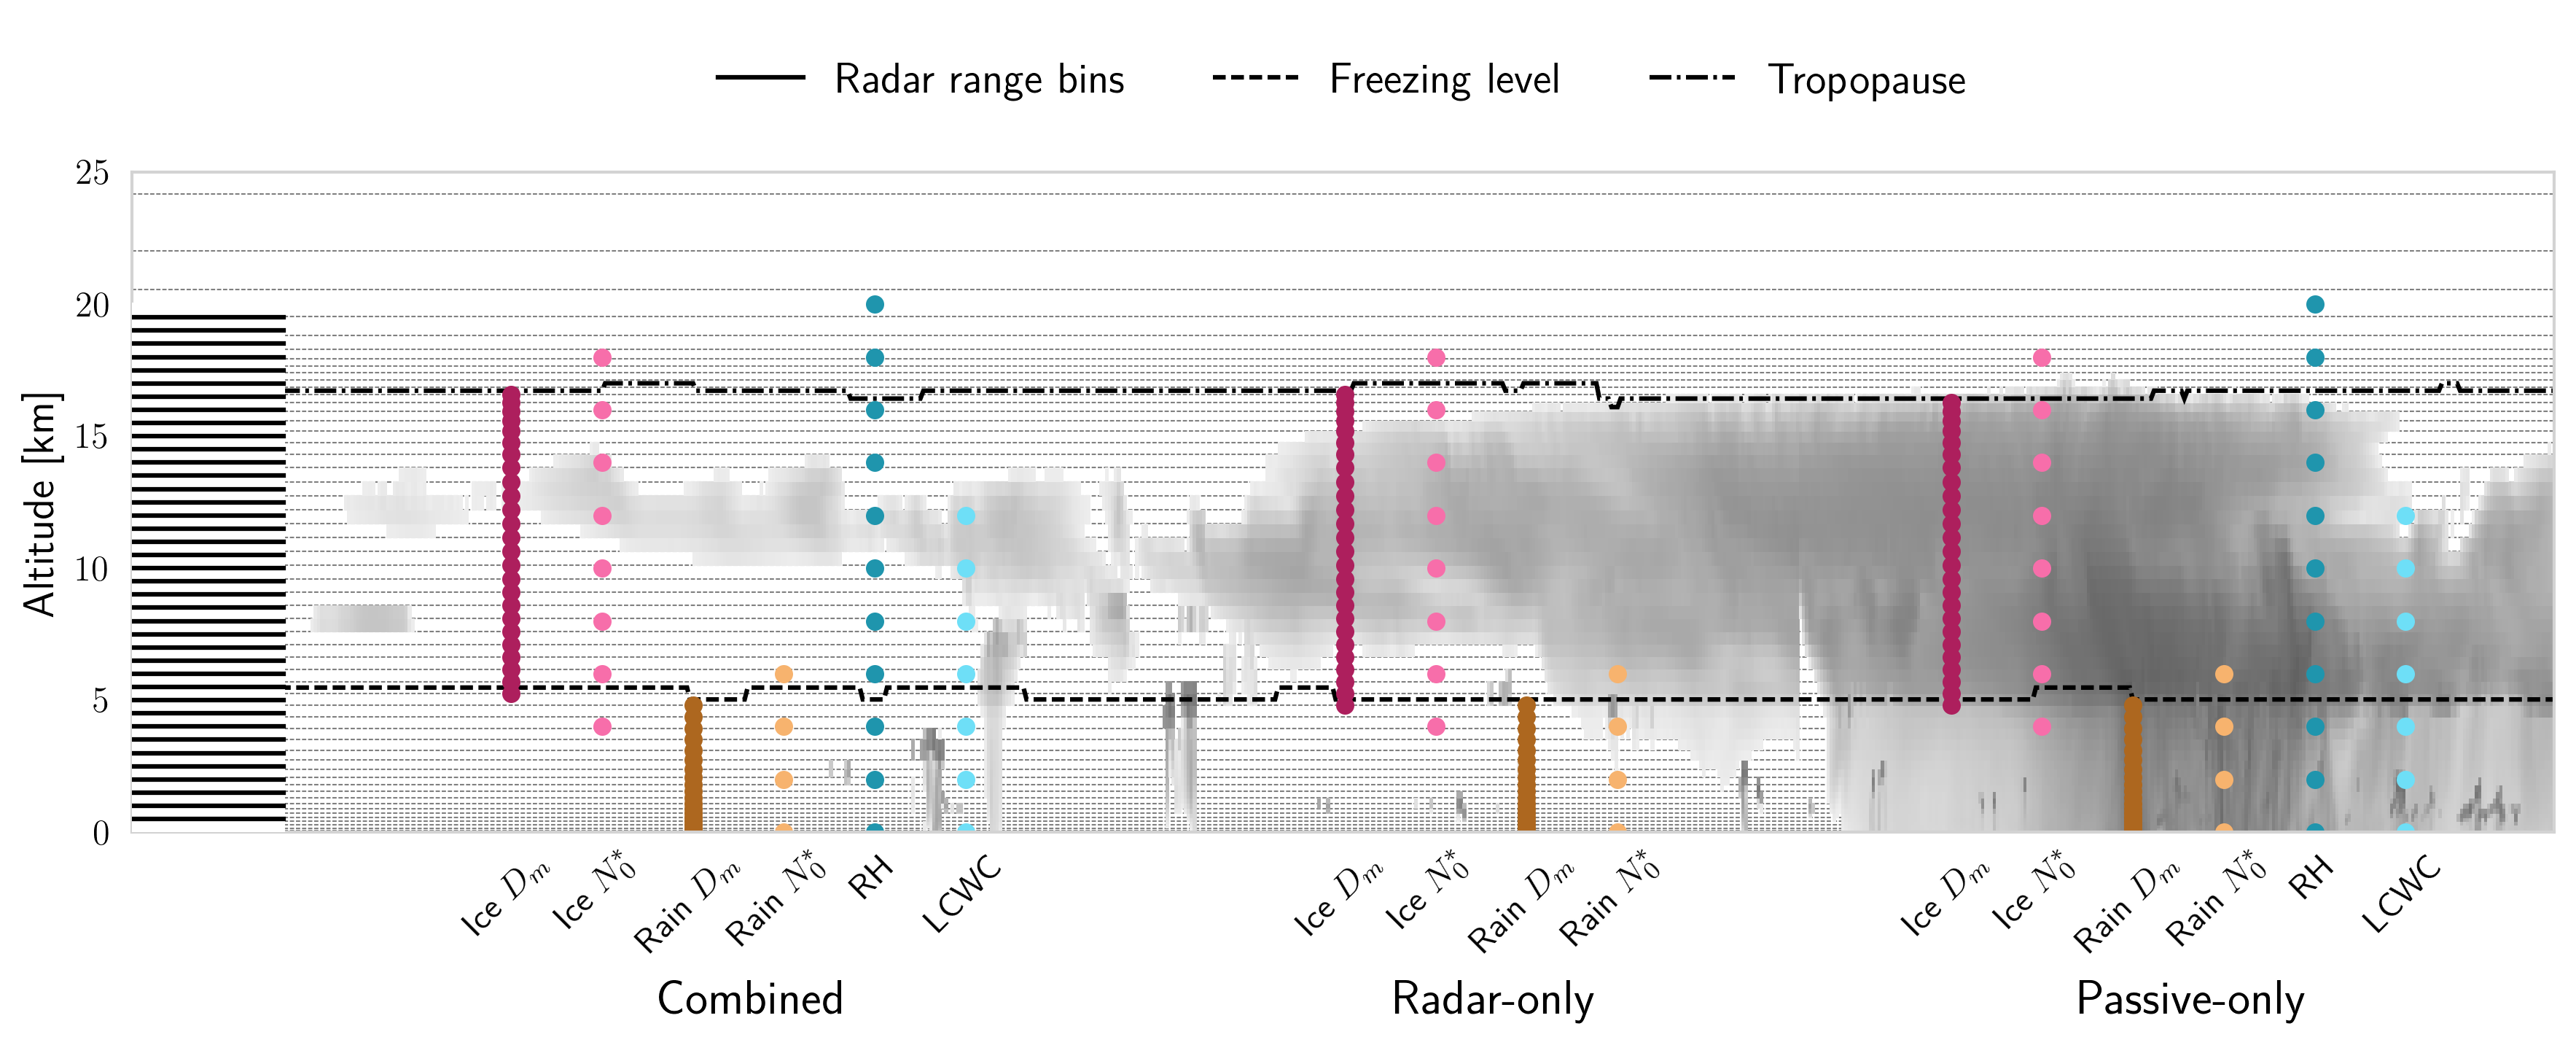
\includegraphics[width = 1.0\linewidth]{../plots/retrieval_sketch}
\caption{Illustration of retrieval quantities and their respective retrieval
  grids. Grey, dashed lines in the background display the vertical grid of the
  GEM model. Black, solid lines on the left side display the range bins of the
  radar observations. Filled markers represent the retrieval grids of each
  retrieval quantity for the combined, radar-only and passive-only
  configurations of the retrieval algorithm.}
\label{fig:retrieval_sketch}
\end{figure}


%To make
%this more clear the following sketch will be added in the beginning of the
%section describing the retrieval setup:

%  \begin{figure}
%\begin{center}
%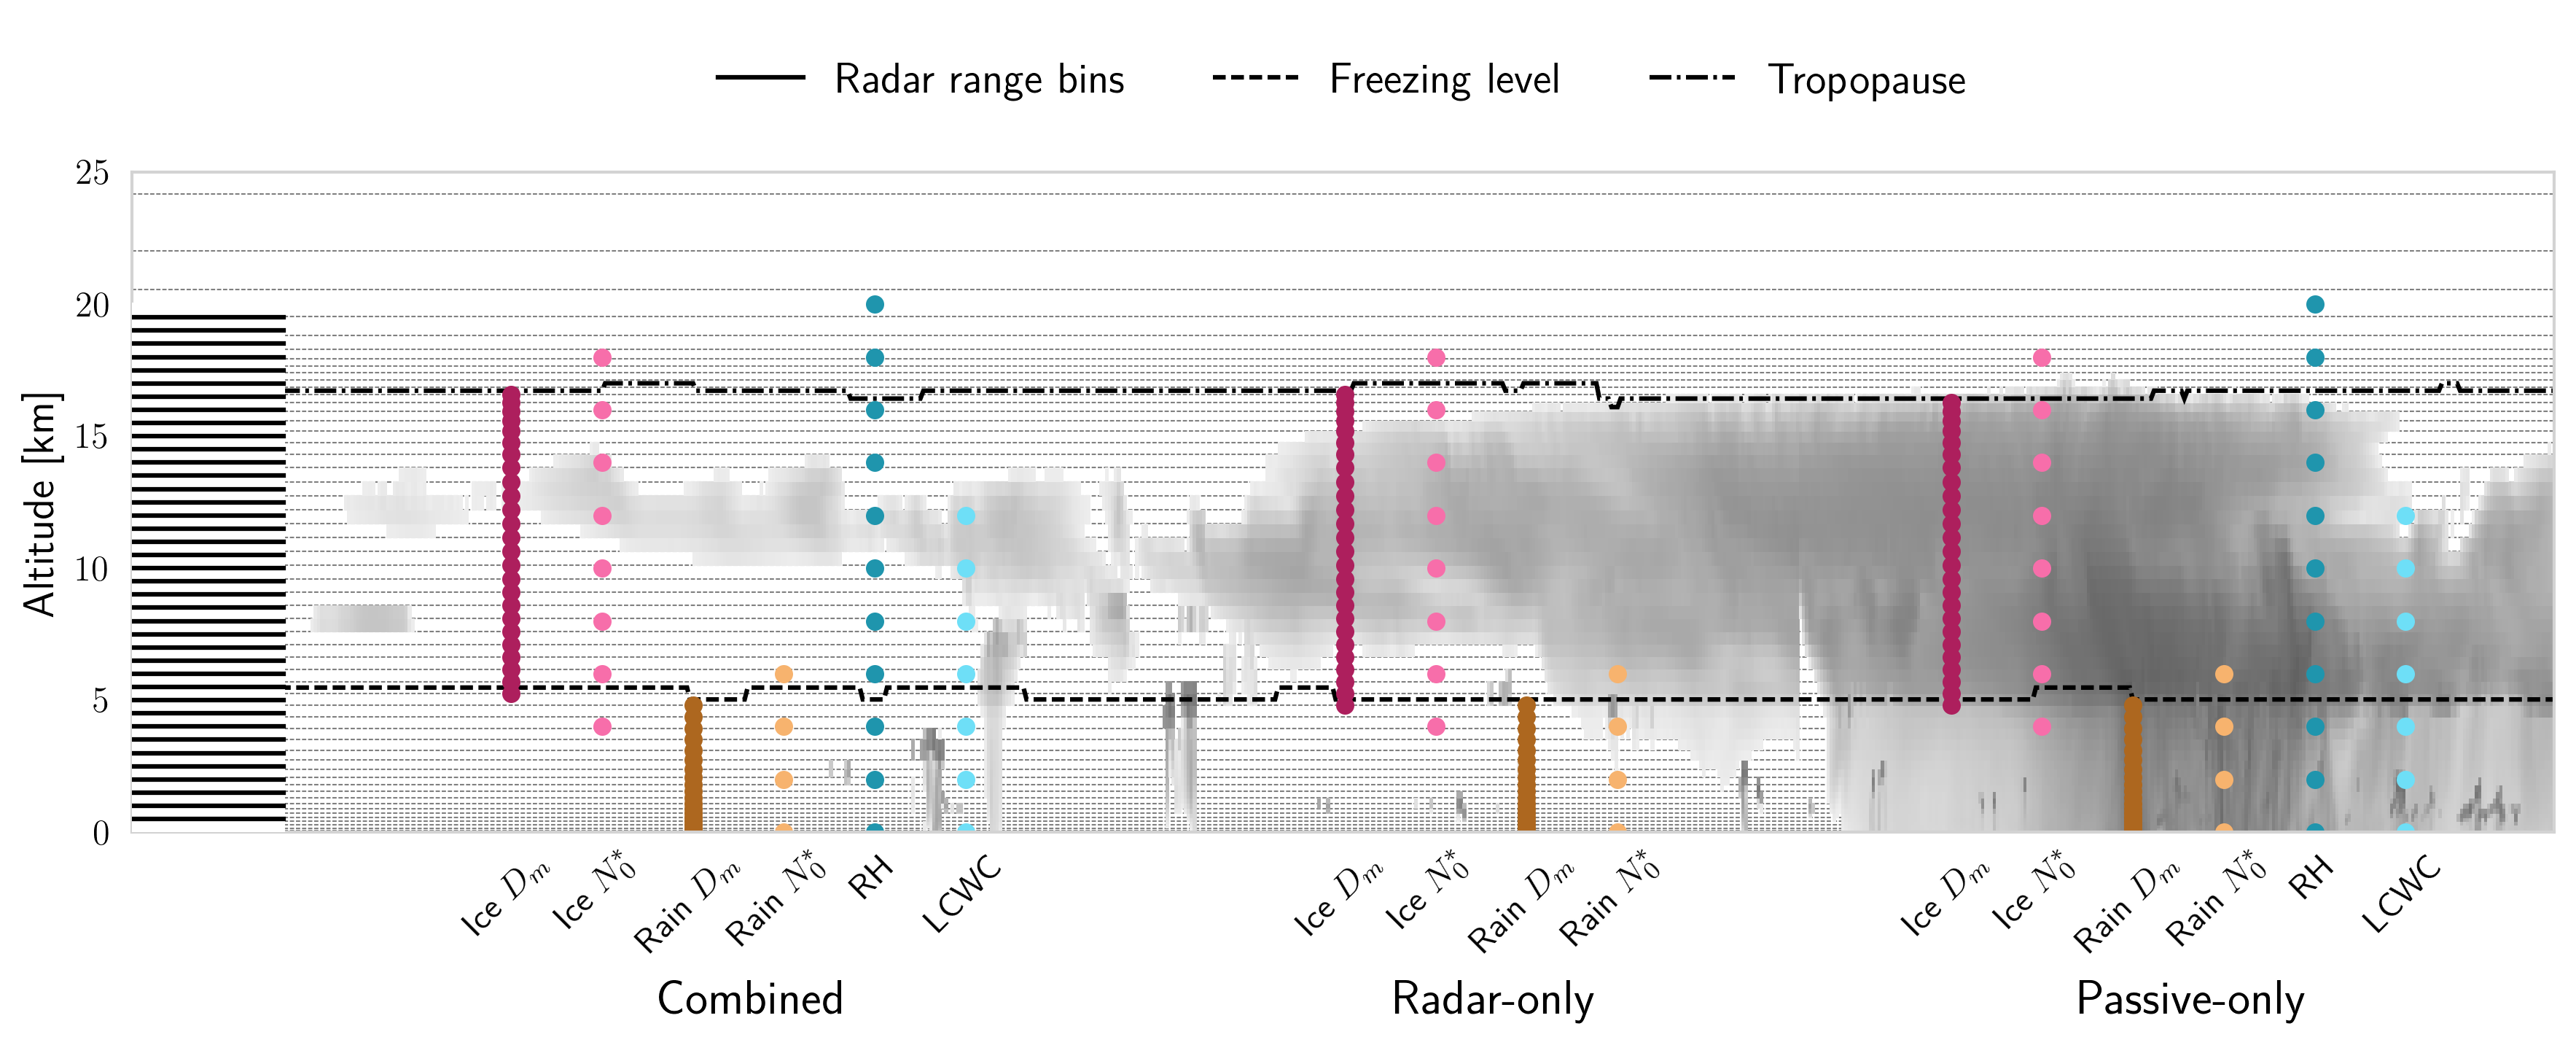
\includegraphics[width = 1.0\linewidth]{../plots/retrieval_sketch}
%\caption{\DIFaddFL{Illustration of the retrieval quantities and their respective retrieval
%  grids. Grey, dashed lines in the background display the vertical grid of the GEM
%  model.  Filled markers represent the retrieval grids of each retrieval quantity
%  for the combined, radar-only and passive-only retrieval.}}
%\label{fig:retrieval_sketch}
%\end{center}
%\end{figure}

\subsection*{Reviewer comment 7}

7. Line 256: Actually, this is only one example of how the radar and radiometer
measurements can be complementary. Even if the lines were parallel (and thus no
information distinguishing size from concentration could be obtained), the radar
still locates the cloud and describes its vertical structure. One can imagine a
cloud of the same ice water path and particle size at two different heights
having different brightness temperatures due to changes in the water vapor
absorption above the cloud – having the radar information would provide
increased information content about the ice water pathin this case than the
radiometer measurement alone.

\subsubsection*{Author response}

It is certainly correct that when a radar sensor is added to a passive
observation system one of the advantages will be the increased resolution.
However, what we are interested in are the advantages that neither of the two
instruments can provide on its own. If it was only about vertical resolution,
then the radar alone would be the ideal observation system. In this sense, we do
not consider the vertical resolution a synergy of the two sensors.

To make this clear, we will add an explanation of our definition of synergies
between the active and passive observations to the section which discusses the
complementary information content.

\subsubsection*{Changes in manuscript}
\begin{change}[237]
A fundamental question regarding the benefit of combining two remote sensing
observations in a retrieval is to what extent the observations contain
non-redundant information. The degree of non-redundancy in the combined
observations is what we refer to here as complementary information content. \DIFaddbegin \DIFadd{We
are thus interested in the information that cannot be provided by either of the
instruments alone. The higher resolution achieved by adding radar observations
to passive ones is therefore not considered as complementary information since
the radar alone can provide the increased resolution.
}
\end{change}

%Although this is certainly one advantage of combining radar and radiometer
%observations, we do not consider this a true synergy of the active and passive
%observations since correctly locating the cloud in the atmosphere is something
%that the radar can do alone. For the passive to add benefit to the radar, the
%combined observations must provide additional information on the microphysics
%that the radar alone does not provide.


\subsection*{Reviewer comment 8}

Table 4: Why are the values for GemSnow and GemGraupel different than in Table 1?

\subsubsection*{Author response}

This was by mistake and has been corrected in the revised version of the
manuscript.

\subsubsection*{Changes in manuscript}

Tables 1 and 4 have been corrected and extended in the revised version
of the manuscript.
%The differences in the reported values for GemSnow and GemGraupel were due to a
%mistake made by the authors. In the revised version of the manuscript this will
%be corrected and, upon recommendation by reviewer 2, merged into a single table.
%The table now looks as follows:
%
%\begin{table}
%  \begin{center}
%  \caption{\DIFaddFL{Particle model name, ARTS scattering database ID and parameters
%    $\alpha, \beta$ of the mass-size relationships of the particle habits used
%    in the retrieval.}}
%  \begin{tabular}{l|c|c|c}
%    \DIFaddFL{Name }& \DIFaddFL{ID }& \DIFaddFL{$\alpha$ }& \DIFaddFL{$\beta$ }\\
%    \hline
%    \DIFaddFL{LiquidSphere }& \DIFaddFL{25 }& \DIFaddFL{523.6 }& \DIFaddFL{3 }\\
%    \DIFaddFL{GemCloudIce          }& \DIFaddFL{11  }& \DIFaddFL{440      }& \DIFaddFL{3 }\\
%    \DIFaddFL{GemSnow              }& \DIFaddFL{32  }& \DIFaddFL{24  }& \DIFaddFL{2.86 }\\
%    \DIFaddFL{GemGraupel           }& \DIFaddFL{33  }& \DIFaddFL{172.7527 }& \DIFaddFL{2.9646 }\\
%    \DIFaddFL{GemHail              }& \DIFaddFL{34  }& \DIFaddFL{3.02 }& \DIFaddFL{2.9646 }\\
%    \hline
%    \DIFaddFL{SectorSnowflake      }&  \DIFaddFL{3 }& \DIFaddFL{0.0008   }& \DIFaddFL{1.44 }\\
%    \DIFaddFL{8-ColumnAggregate    }&  \DIFaddFL{8   }& \DIFaddFL{65       }& \DIFaddFL{3 }\\
%    \DIFaddFL{LargeColumnAggregate }&  \DIFaddFL{18 }& \DIFaddFL{0.25     }& \DIFaddFL{2.43 }\\
%    \DIFaddFL{LargePlateAggregate  }&  \DIFaddFL{20 }& \DIFaddFL{0.21     }& \DIFaddFL{2.26 }\\
%    \DIFaddFL{IceSphere            }&  \DIFaddFL{24 }& \DIFaddFL{2.2571   }& \DIFaddFL{0.2085 }\\
%  \end{tabular}
%  \label{tab:particle_properties}
%\end{center}
%\end{table}

\subsection*{Reviewer comment 9}

Figures 7 and 8:  I’m not sure why these are separate figures – it seems like all panels could fit on one page.

\subsubsection*{Author response}

Figures 7 and 8 have been combined into a single figure in the revised
manuscript.


\subsubsection*{Changes in manuscript}

Figures 7 and 8 have been combined into a single figure and now look as shown in
Fig.~\ref{fig_scatter_a}.

\begin{figure}
\centering 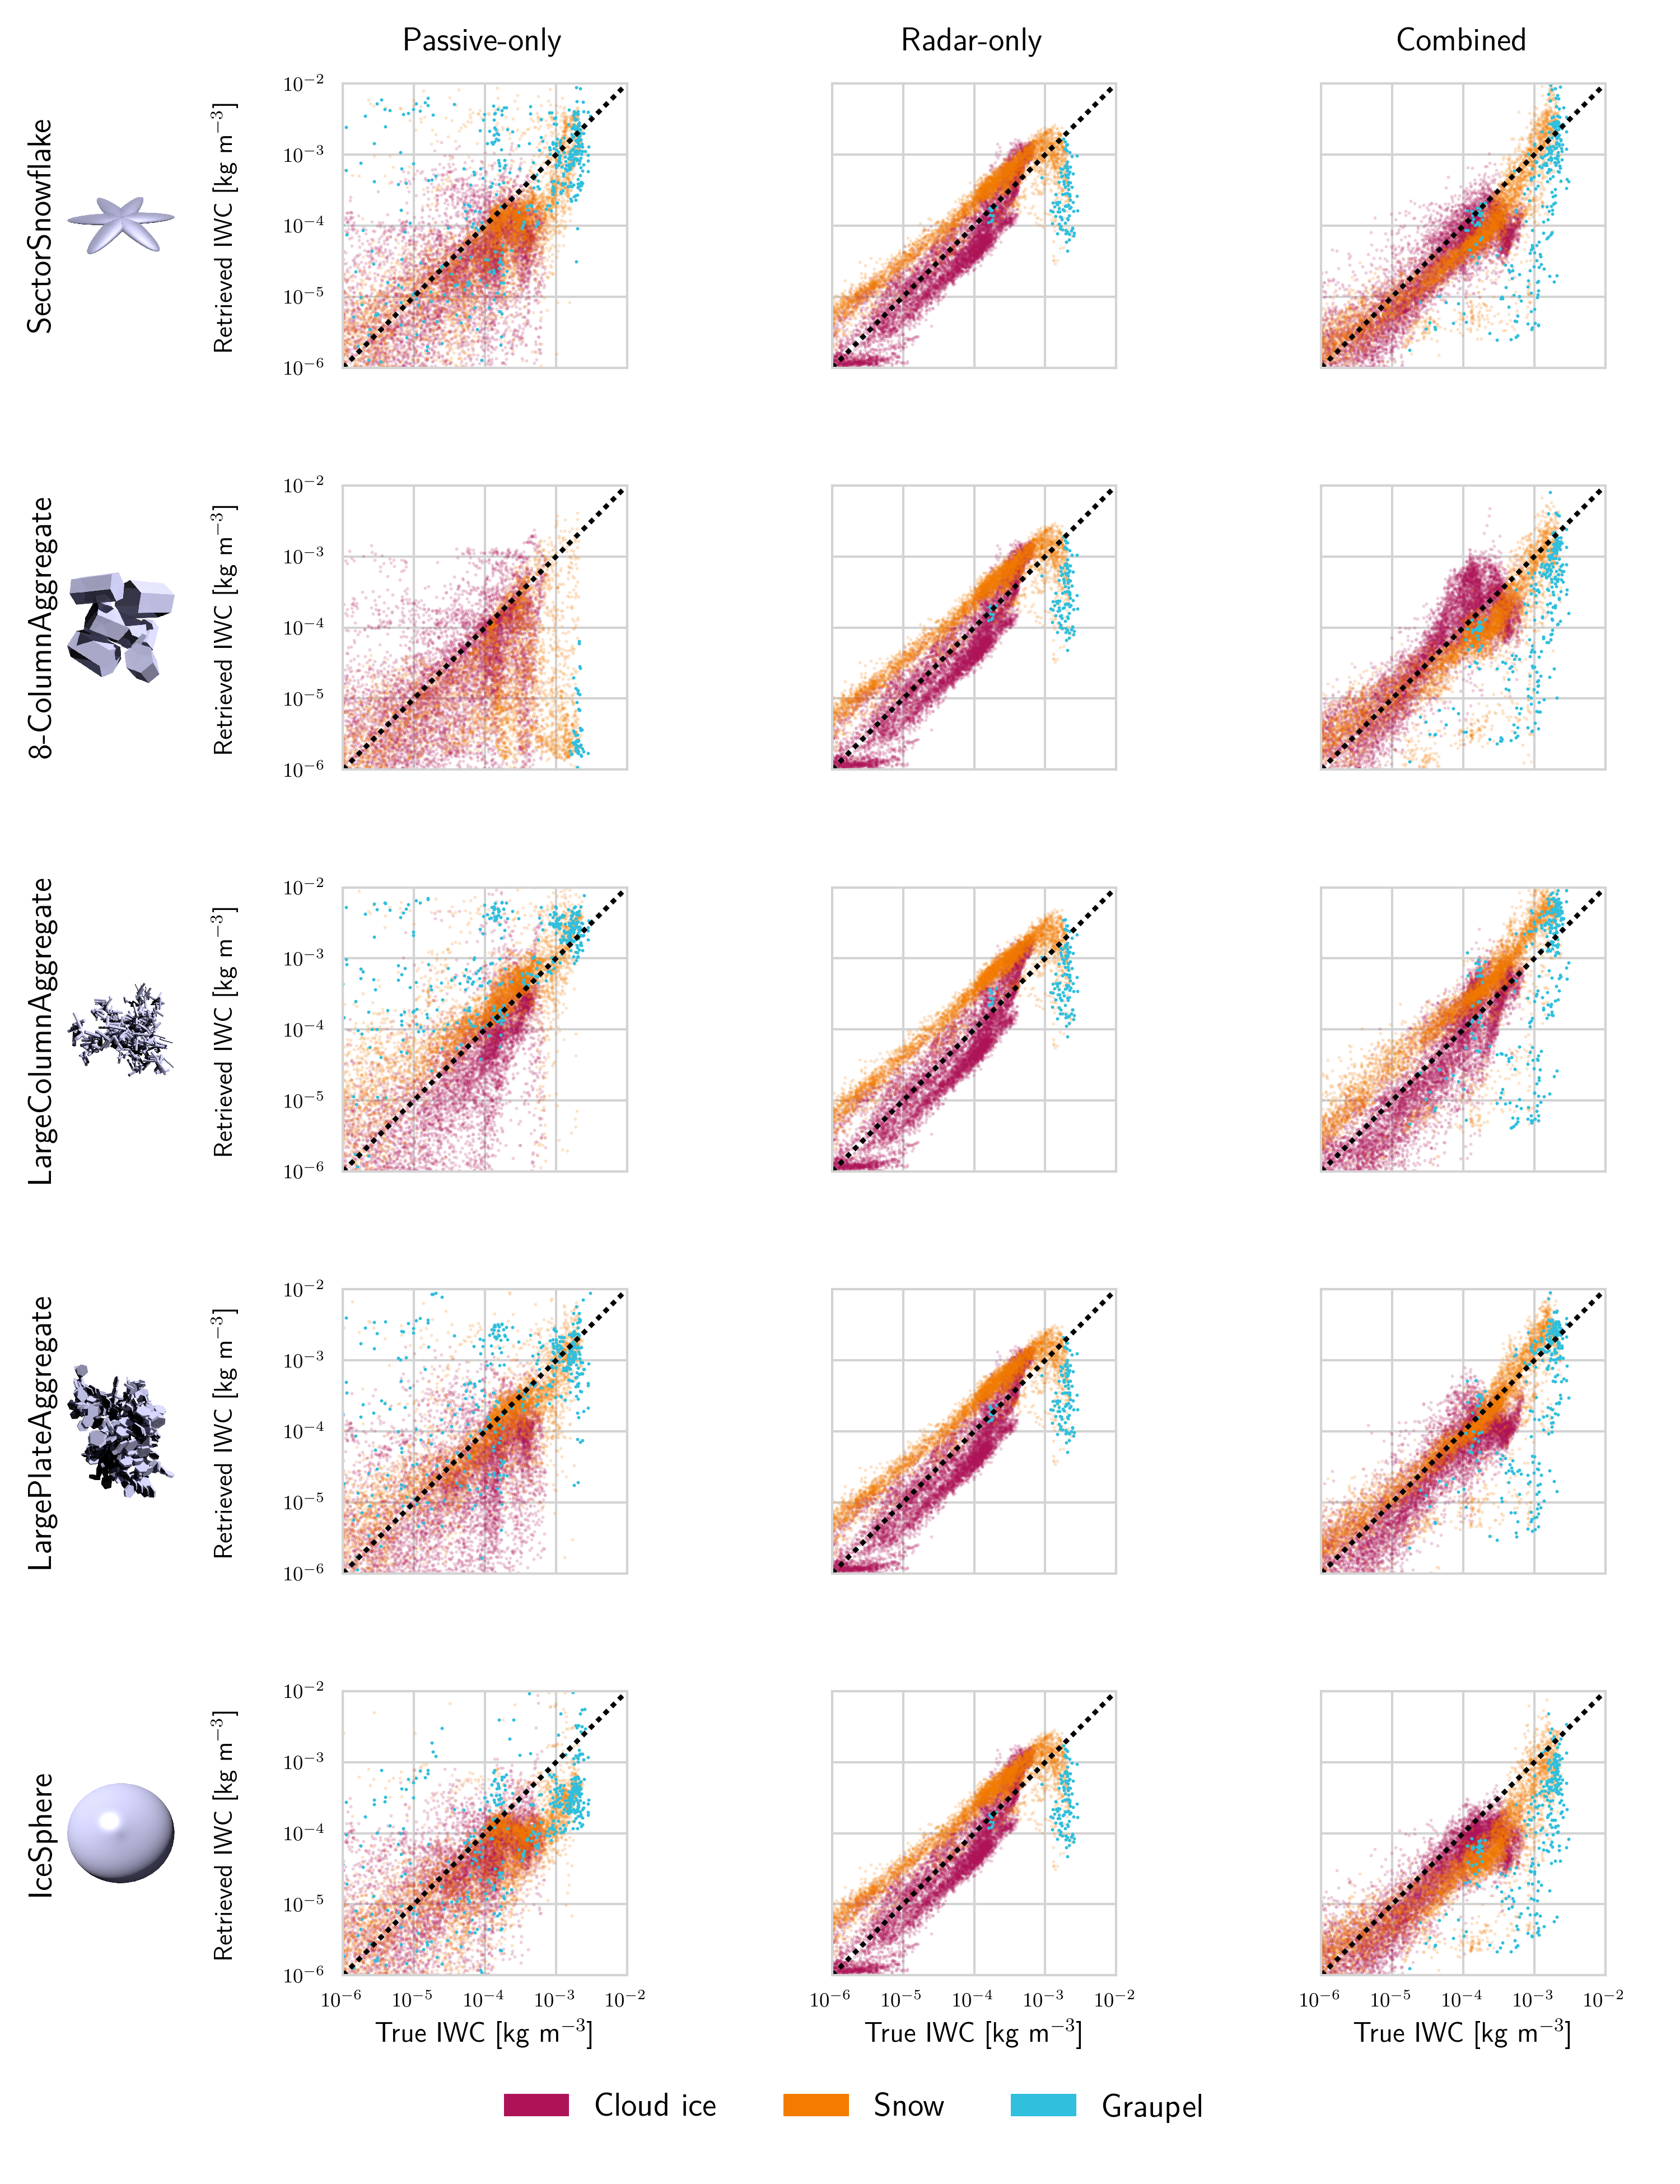
\includegraphics[width = 0.75\textwidth]{../plots/results_scatter_a}
\caption{Retrieved IWC plotted against reference IWC for the tested retrieval
  configurations. Each row shows the retrieval results for the particle shape
  shown in the first panel. The following panels show the retrieval results for
  the passive-only (first column), the radar-only (second column) and the
  combined retrieval (third column). Markers are colored according to the
  prevailing hydrometeor type at the corresponding grid point in the test
  scene. Due to their sparsity, markers corresponding to graupel are drawn at
  twice the size of the other markers.}
\label{fig:results_scatter_a}
\end{figure}

\subsection*{Reviewer comment 10}

Figure 10 is missing from the manuscript.

\subsubsection*{Author response}

Figure 10 has been included in an Appendix to the revised manuscript with the
rest of the analysis of the results from the second test scene.

\subsubsection*{Changes in manuscript}

The figure shown in Fig.\ref{fig:results_scatter_b} has been added in the appendix
of the manuscript.

\begin{figure}[!h]
\centering
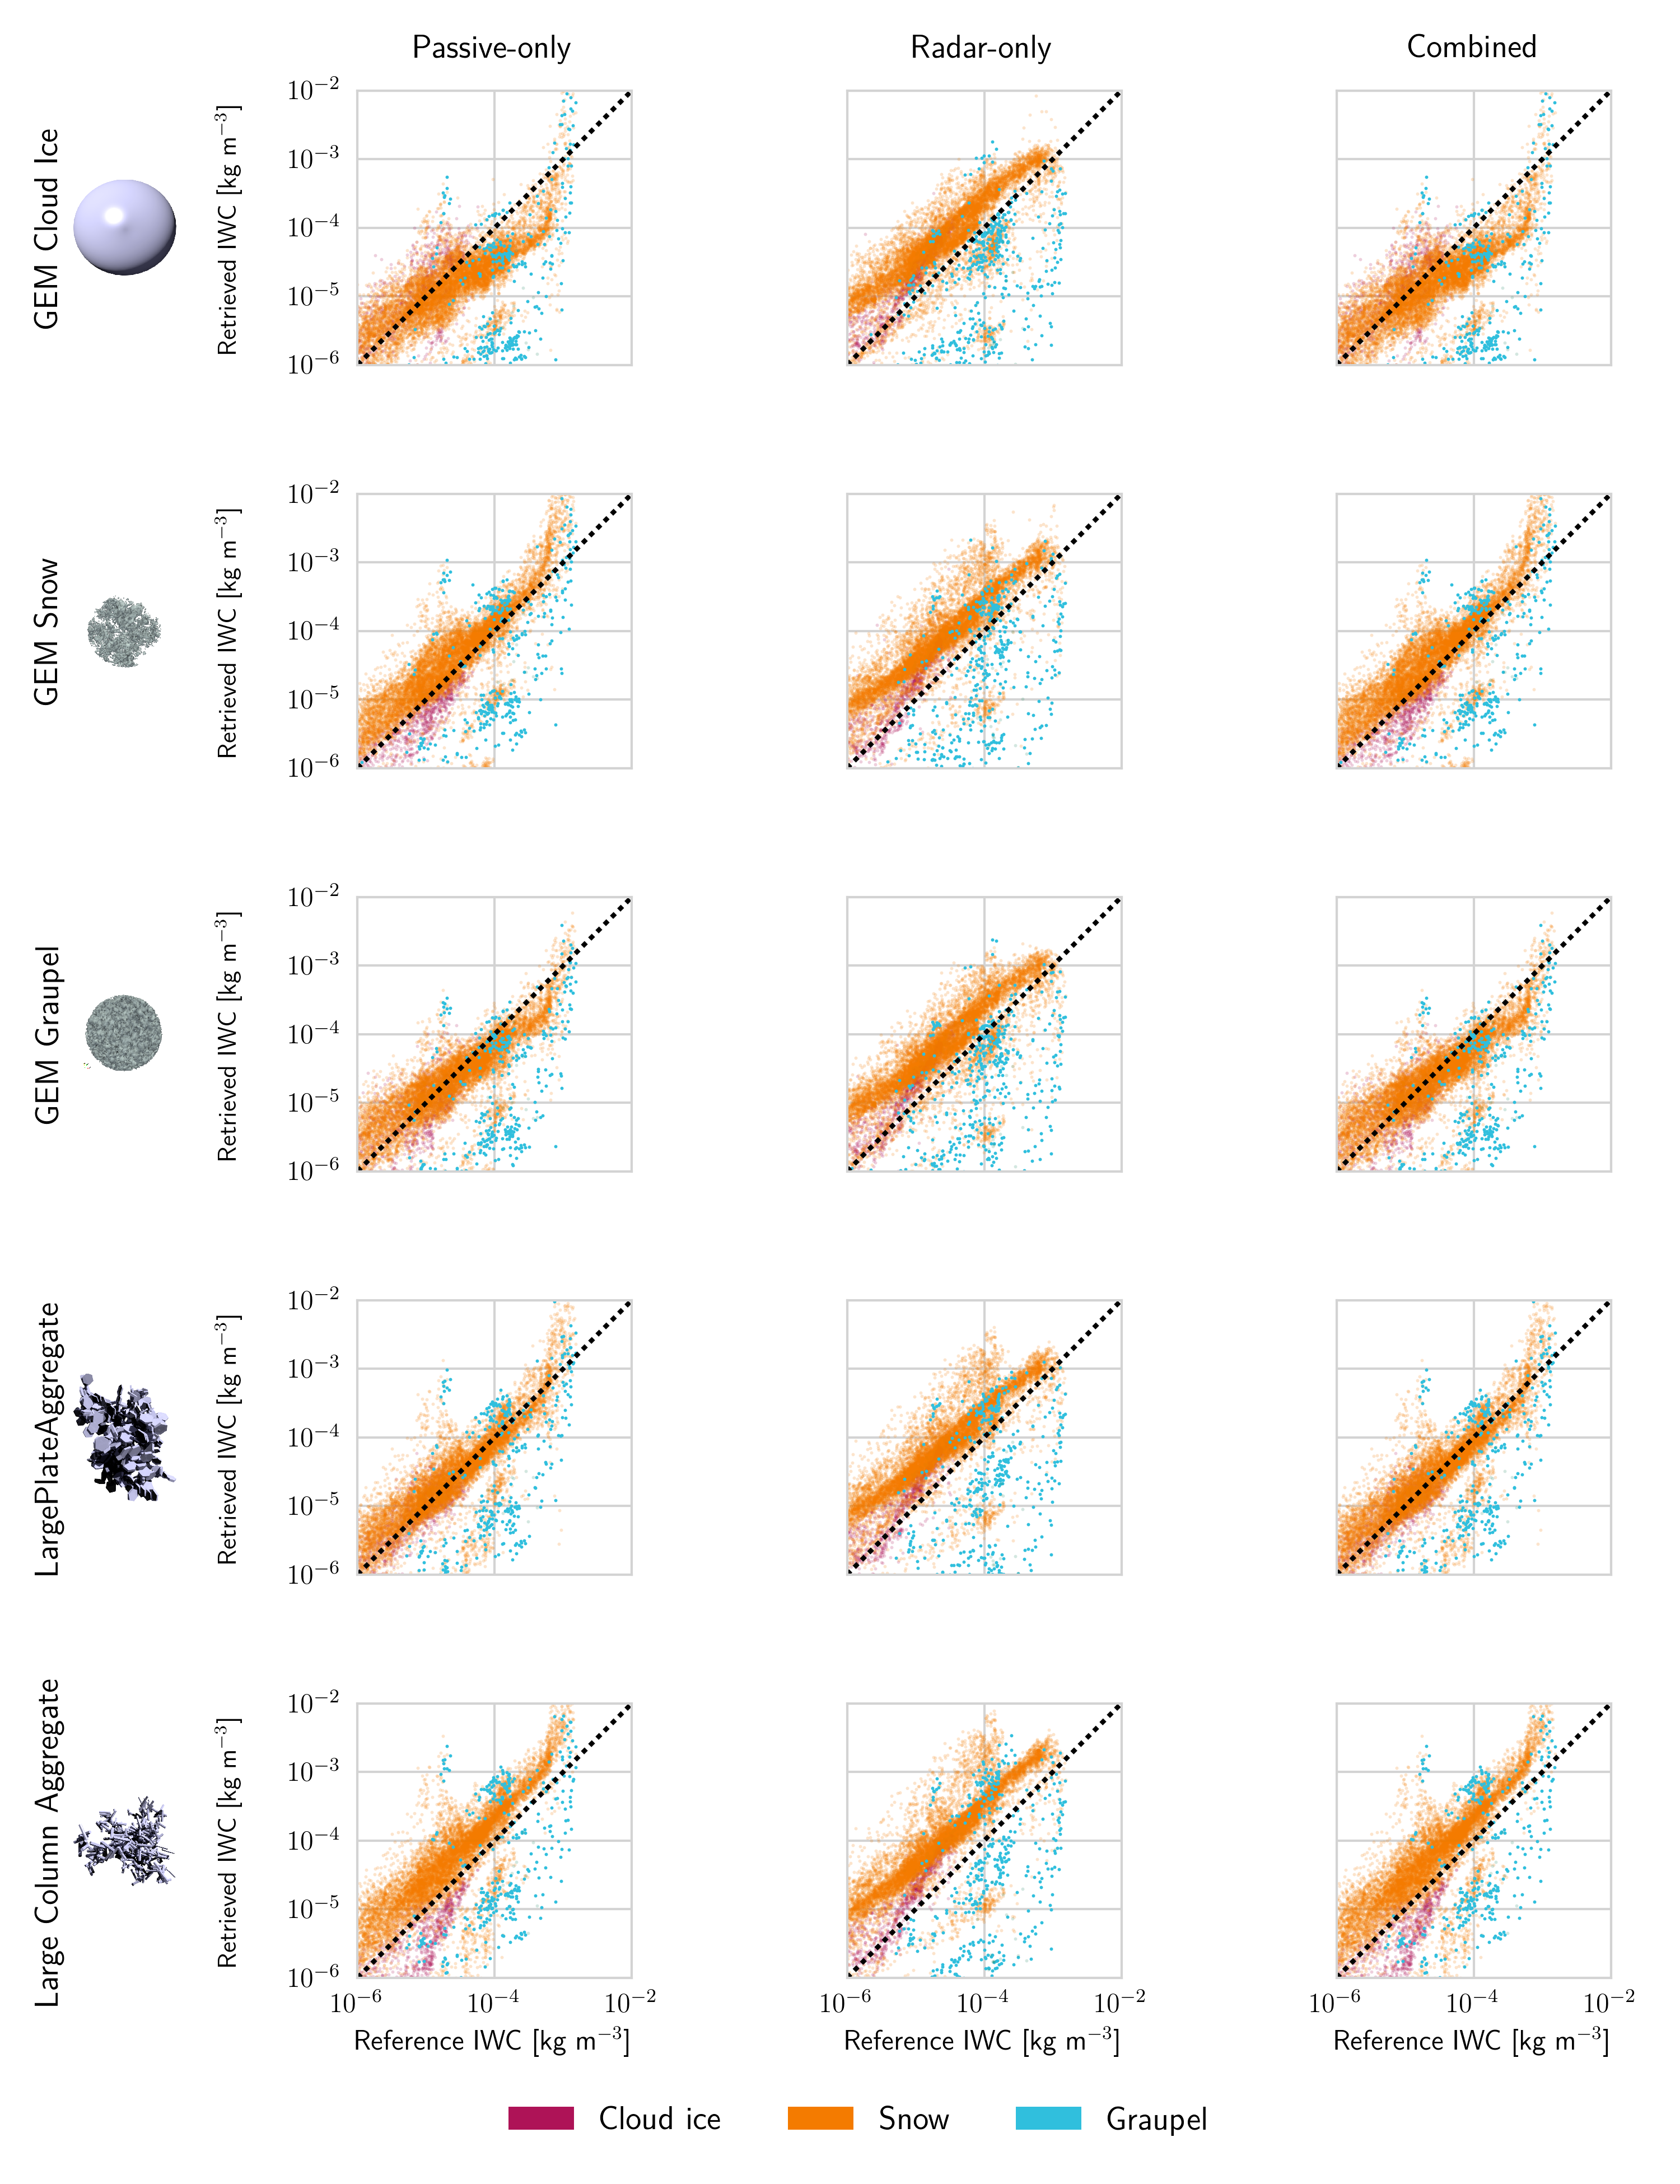
\includegraphics[width = 0.8\textwidth]{../plots/results_scatter_b}
\caption{Scatter plots of the reference and retrieved IWC for
  the second test scene. The rows show the retrieval results for a given
  assumed ice particle model. The first column of each row displays a rendering
  of the particle model. The following rows display the results for the
  passive-only, the radar-only and the combined retrieval.}
\label{fig:results_scatter_b}
\end{figure}




%The figure 7 and 8 will be combined into a single figure in the revised version
%of the manuscript:
%
%\begin{figure}
%\begin{center} \DIFdelbeginFL %DIFDELCMD < \includegraphics[width = 0.8\textwidth]{figures/fig07}
%%DIFDELCMD < %%%
%\DIFdelendFL \DIFaddbeginFL 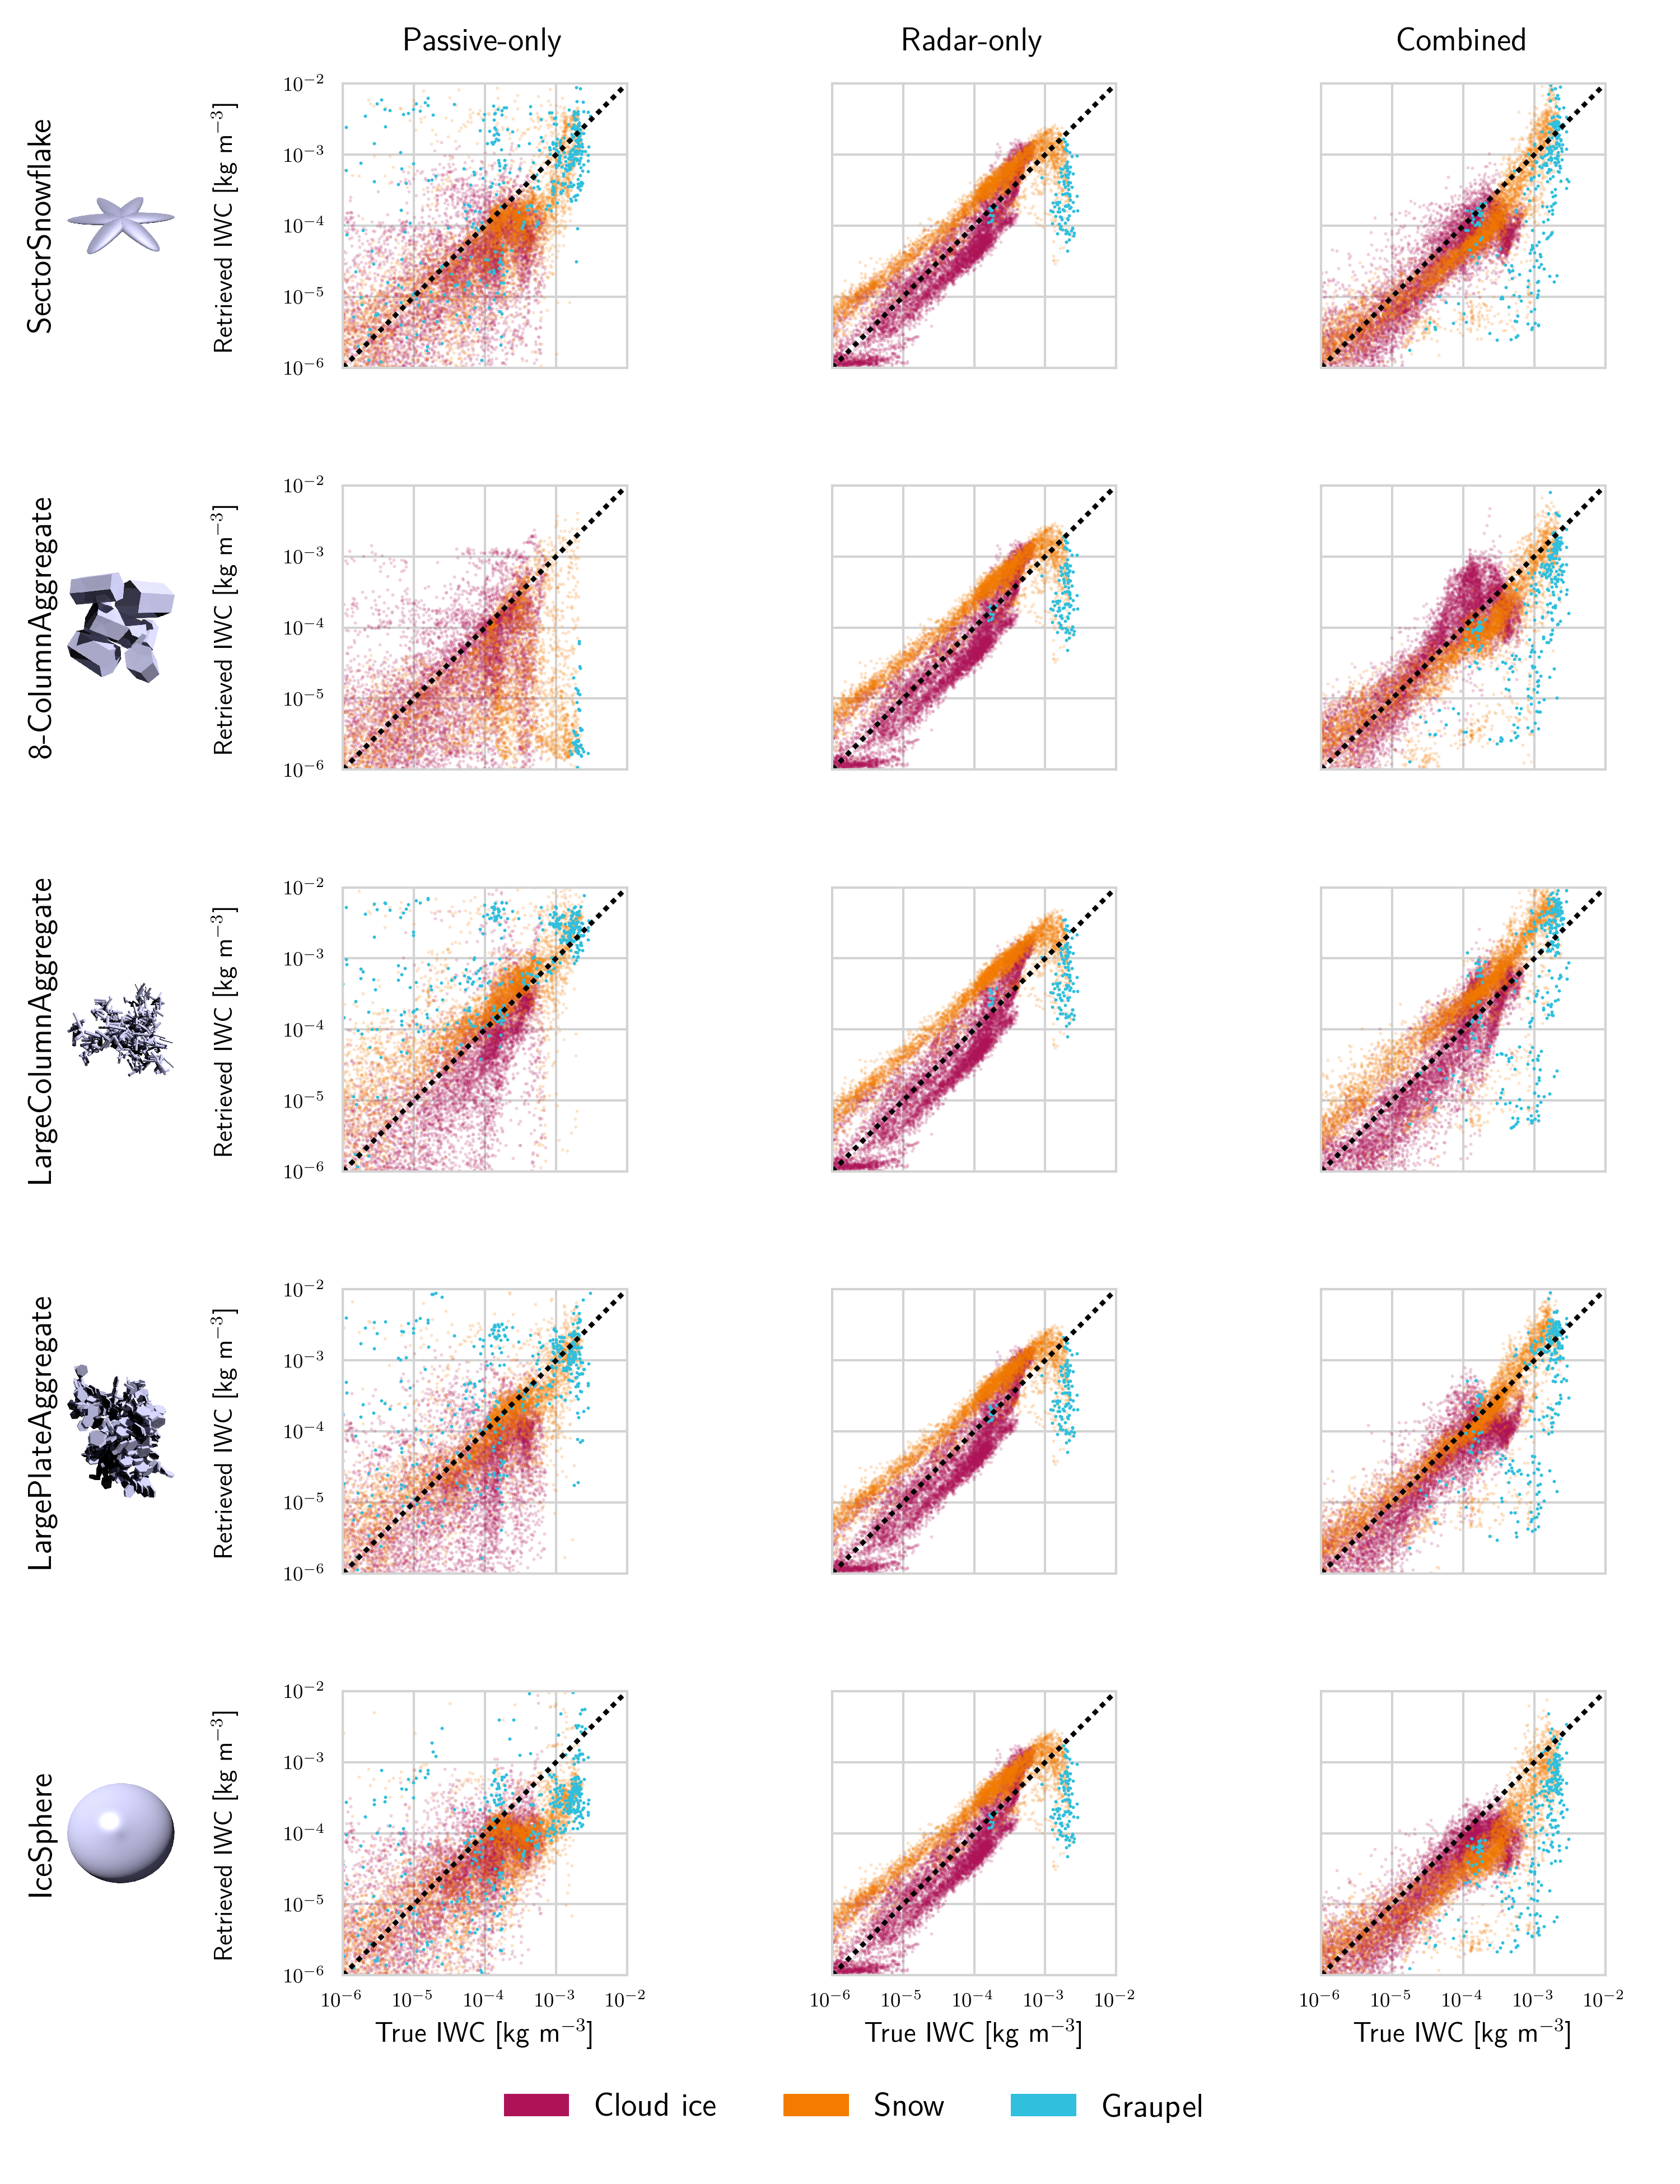
\includegraphics[width = 0.75\textwidth]{../plots/results_scatter_a}
%\DIFaddendFL \caption{\DIFdelbeginFL \DIFdelFL{Reference }\DIFdelendFL \DIFaddbeginFL \DIFaddFL{Retrieved }\DIFaddendFL IWC plotted against \DIFdelbeginFL \DIFdelFL{retrieved }\DIFdelendFL \DIFaddbeginFL \DIFaddFL{reference }\DIFaddendFL IWC for the tested retrieval
%  configurations. Each row shows the retrieval results for the particle shape
%  shown in the first panel. The following panels show the retrieval results for
%  the passive only (first column), the radar only (second column) and the
%  combined retrieval (third column). Markers are colored according to the
%  prevailing hydrometeor type at the corresponding grid point in the test
%  scene. Due to their sparsity, markers corresponding to graupel are drawn at
%  twice the size of the other markers.}
%\DIFdelbeginFL %DIFDELCMD < \label{fig:results_scatter_a_1}
%%DIFDELCMD < %%%
%\DIFdelendFL \DIFaddbeginFL \label{fig:results_scatter_a}
%\DIFaddendFL \end{figure}
%\end{center}

\subsection*{Reviewer comment 11}
 Line 374: recommend using “represent” instead of “predict”

\subsubsection*{Author response}

The proposed change has been adopted in the revised version of the manuscript.

\subsubsection*{Changes in manuscript}

\begin{change}[374]
 Since snow will have \DIFdelbegin \DIFdel{the
}\DIFdelend \DIFaddbegin \DIFadd{a }\DIFaddend stronger impact on the
observations, the retrieval in these regions \DIFdelbegin \DIFdel{tends to predict }\DIFdelend \DIFaddbegin \DIFadd{will likely tend to represent }\DIFaddend snow
rather than ice, which leads to the low retrieved number \DIFdelbegin \DIFdel{densities}\DIFdelend \DIFaddbegin \DIFadd{concentrations}\DIFaddend .
\end{change}

%\begin{change}[374]
%Since snow will have the
%stronger impact on the observations, the retrieval in these regions tends to
%\DIFdelbegin \DIFdel{predict }\DIFdelend \DIFaddbegin 
%\end{change}

\subsection*{Reviewer comment 12}

 Line 382: should be “reference” instead of “references”

\subsubsection*{Author response}
This has been corrected in the updated version of the manuscript.

\subsubsection*{Changes in manuscript}
 \begin{change}[382]
The radar-only retrieval does not
exhibit any retrieval skill, hardly reproducing any of the variation of the
\DIFdelbegin \DIFdel{references }\DIFdelend \DIFaddbegin \DIFadd{reference }\DIFaddend values.
 \end{change}

\subsection*{Reviewer comment 13}

Line  414:  How  are  the  truncated  PSDs  (using  GemSnow)  represented  in  theforward simulations? Is total ice water content conserved? If so, how is it spread amongthe valid particle sizes – equally, or is the truncated mass allocated to the smallest size bin?

\subsubsection*{Author response}

Total IWC is not conserved in the handling of PSDs. The point raised by the reviewer has been
investigated by assessing the effect of the truncation on the water content of snow in the
forward simulations. The results of the analysis are given in the figure below. As these results
show, the effects of the truncation in the forward simulations are negligible.

However, when the GemSnow particle model is used in the retrieval it can
introduce significant errors. For this reason as well as another reviewers'
comment regarding the choice of tested particles, the selection of particles to
be used in the retrieval will be changed for the revised manuscript and the
GemSnow particle will be replaced by a habit mix which uses the GemSnow
particle for large diameters.

\begin{figure}[!hbpt]
  \begin{center}
  \includegraphics[width = 1.0\textwidth]{../plots/truncated_iwc}
  \caption{Joint distribution of truncated and full snow water content (SWC) for the
    two test scenes.}
  \end{center}
\end{figure}

\subsection*{Reviewer comment 14}

Figure 16: The figure labels/captions aren't clear if they refer to total liquid
water content/path or just the cloud liquid water/path.

\subsubsection*{Author response}

We will clarify that the contours refer to liquid cloud water content in the
revised version of the manuscript.

\subsubsection*{Changes in manuscript}

To make clear what the labels refer to, they have been changed to liquid cloud
water content (LCWC) in the figure. The new figure is shown in Fig.~\ref{fig:results_cw_b}.

\begin{figure}
\centering
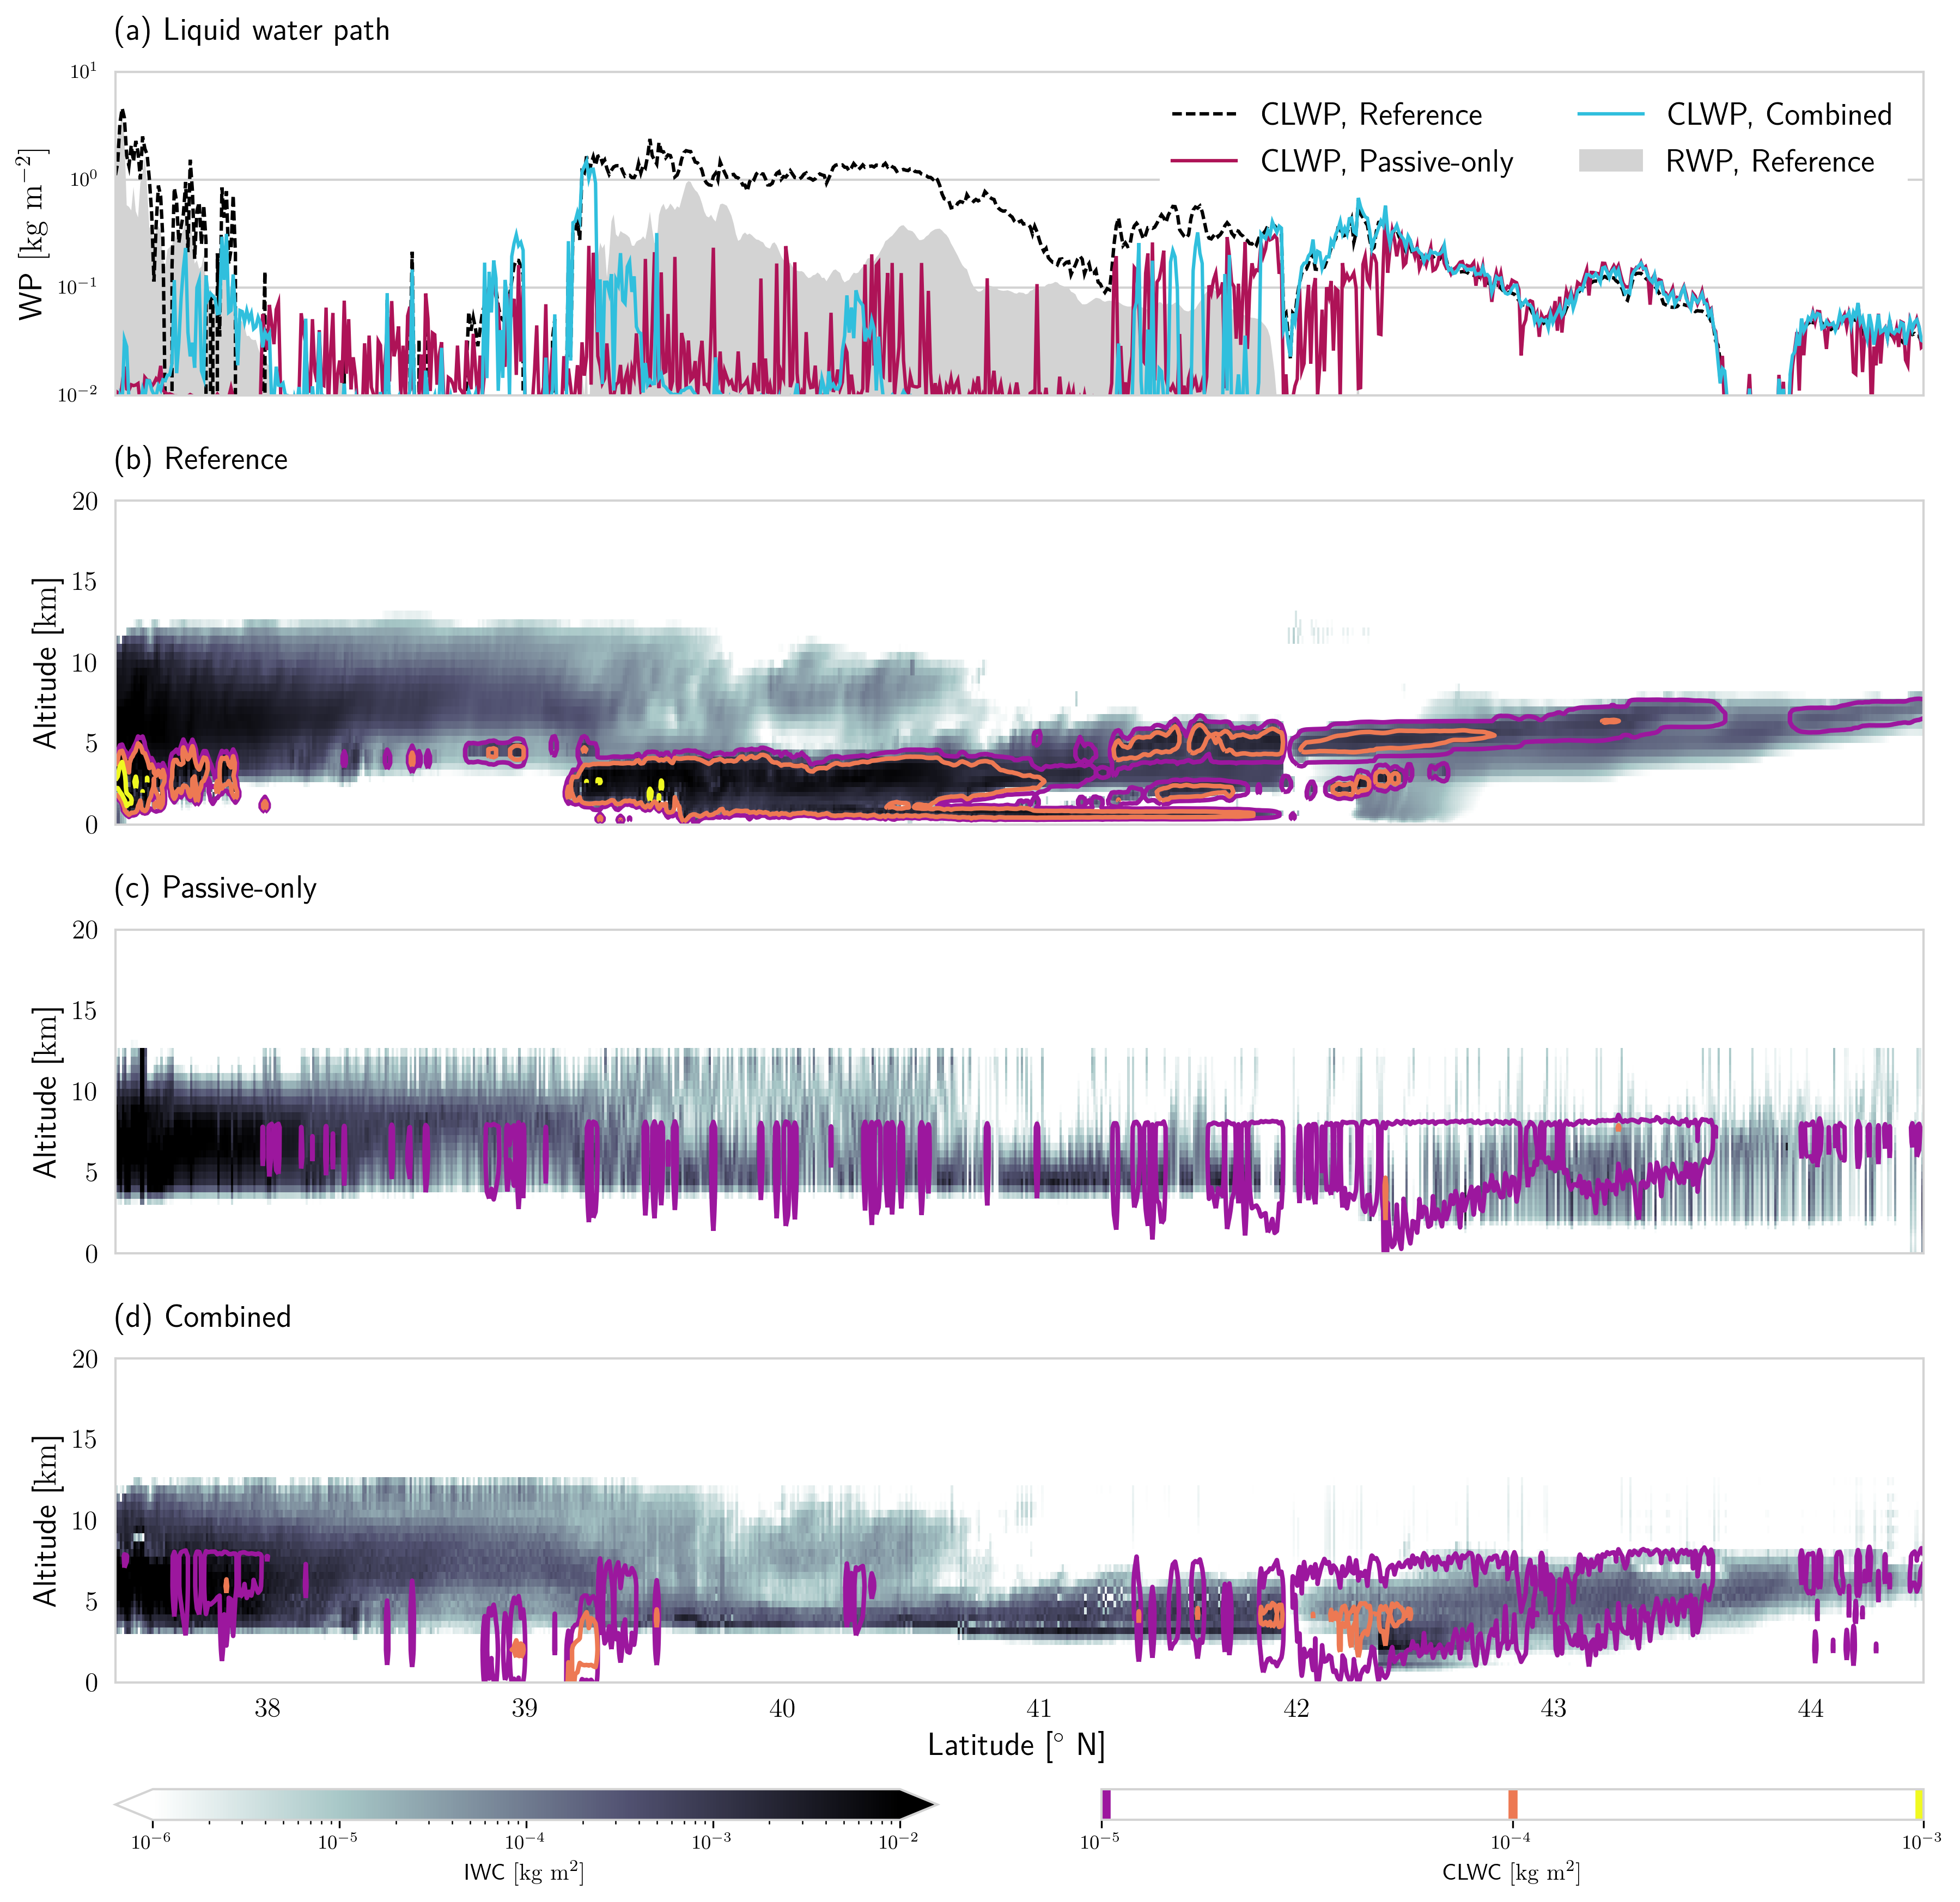
\includegraphics[width = \textwidth]{../plots/results_cw_b_LargePlateAggregate}
\caption{Reference and retrieved CLWC and IWC. Panel (a) shows the reference and
  retrieved LWP for each profile. Panel (b) displays reference LWC contours
  drawn on top of the total hydrometeor content. Retrieval results for
  passive-only and combined retrieval are given in Panel (c) and (d).}
\label{fig:results_cw_b}
\end{figure}

\subsection*{Reviewer comment 15}

 Line 518: It’s interesting that the Plate Aggregate provides the most accurate
 re-trieval results, even though it isn’t similar to the models used in the
 synthetic measurement simulations. Does the decreasing density with size
 better replicate the combina-tion of high-density GemCloudIce (which tends to
 be present in high concentrations atsmall sizes) and lower-density GemSnow
 (which tends to be dominant at larger sizes)?

\subsubsection*{Author response}

Unfortunately, we cannot give a definitive answer to this question. As panel (a)
in Fig. 15 shows, the density of the LargePlateAggregate habit is actually lower
than that of snow for large particle sizes. Moreover, the scattering properties
certainly also play a role here. From these results alone, we are therefore not able to
postulate any direct causality between the particle density and the performance
in the retrieval.

\subsubsection*{Changes in manuscript}

To provide more definitive recommendations regarding the choice of the particle
model, we have reconsidered the selection of models to test and added the figure
shown in Fig.~\ref{fig:particle_properties} to the manuscript. These results
indicate that a potential explanation of the good performance of the Large Plate
Aggregate is that its scattering properties are intermediate to those of
GEM cloud ice and GEM snow.


\begin{figure}
  \centering
  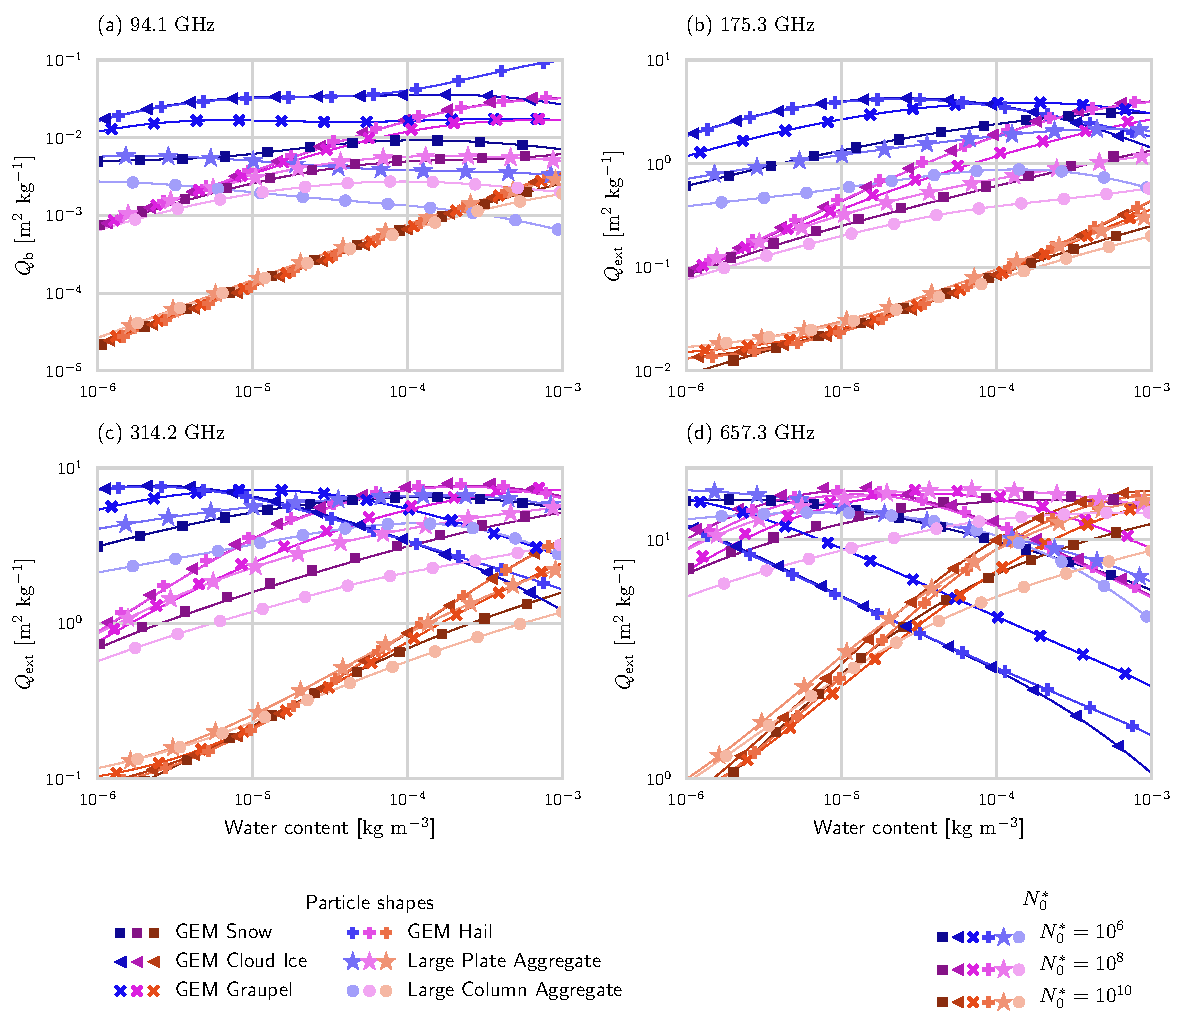
\includegraphics[width=0.8\textwidth]{../plots/particle_properties_d14}
  \caption{Bulk mass backscattering efficiency $Q_b$ at $94.1\ \unit{GHz}$ (a)
    and mass attenuation coefficients $Q_{e}$ at frequencies $175.3\ \unit{GHz}$
    (b), $314.2\ \unit{GHz}$ (c) and $657.3\ \unit{GHz}$ (d) for the particle
    models used in the simulated observations and the retrieval. Different
    colors show the bulk properties for different values of the $N_0^*$
    parameter of the PSD.}
  \label{fig:particle_properties}
\end{figure}
